%% IMPORTANT NOTICE:
%%
%% For the copyright see the source file.
%% This generated file may be distributed as long as the
%% original source files, as listed above, are part of the
%% same distribution. (The sources need not necessarily be
%% in the same archive or directory.)
%%
%% The first command in your LaTeX source must be the \documentclass command.
%%%% Small single column format, used for CIE, CSUR, DTRAP, JACM, JDIQ, JEA, JERIC, JETC, PACMCGIT, TAAS, TACCESS, TACO, TALG, TALLIP (formerly TALIP), TCPS, TDSCI, TEAC, TECS, TELO, THRI, TIIS, TIOT, TISSEC, TIST, TKDD, TMIS, TOCE, TOCHI, TOCL, TOCS, TOCT, TODAES, TODS, TOIS, TOIT, TOMACS, TOMM (formerly TOMCCAP), TOMPECS, TOMS, TOPC, TOPLAS, TOPS, TOS, TOSEM, TOSN, TQC, TRETS, TSAS, TSC, TSLP, TWEB.
% \documentclass[acmsmall]{acmart}

%%%% Large single column format, used for IMWUT, JOCCH, PACMPL, POMACS, TAP, PACMHCI
% \documentclass[acmlarge,screen]{acmart}

%%%% Large double column format, used for TOG
\documentclass[acmtog, authorversion]{acmart}



%%%% Generic manuscript mode
% \documentclass[manuscript,screen,review]{acmart}

%% Rights management information.  This information is sent to you
%% when you complete the rights form.  These commands have SAMPLE
%% values in them; it is your responsibility as an author to replace
%% the commands and values with those provided to you when you
%% complete the rights form.
\setcopyright{acmcopyright}
\copyrightyear{2018}
\acmYear{2018}
\acmDOI{10.1145/1122445.1122456}

%% These commands are for a PROCEEDINGS abstract or paper.
\acmConference[PEARC '20]{Woodstock '18: ACM Symposium on Neural
  Gaze Detection}{June 03--05, 2020}{Portland, OR}

\usepackage{subcaption}
\usepackage{float}

%% end of the preamble, start of the body of the document source.
\begin{document}

%% The "title" command has an optional parameter,
%% allowing the author to define a "short title" to be used in page headers.
\title{Building Detection with Deep Learning}

%% The "author" command and its associated commands are used to define
%% the authors and their affiliations.
%% Of note is the shared affiliation of the first two authors, and the
%% "authornote" and "authornotemark" commands
%% used to denote shared contribution to the research.
%% \authornote{Both authors contributed equally to this research.}

\author{Matthew Kusz}
\email{mkusz@iu.edu}
\affiliation{%
  \institution{Indiana University}
  \city{Bloomington}
  \state{Indiana}
  \postcode{43017-6221}
}

\author{Justin Peters}
\affiliation{%
  \institution{Indiana University}
  \city{Bloomington}
  \state{Indiana}}
  \postcode{43017-6221}
\email{jppeters@iu.edu}

\author{Laura Huber}
\affiliation{%
  \institution{Indiana University}
  \city{Bloomington}
  \state{Indiana}}
  \postcode{43017-6221}
\email{lamhuber@iu.edu}

\author{Jefferson Davis}
\affiliation{%
  \institution{Indiana University}
  \city{Bloomington}
  \state{Indiana}}
  \postcode{43017-6221}
\email{majdavis@iu.edu}

\author{Scott Michael}
\affiliation{%
  \institution{Indiana University}
  \city{Bloomington}
  \state{Indiana}}
  \postcode{43017-6221}
\email{scamicha@iu.edu}

%%
%% By default, the full list of authors will be used in the page
%% headers. Often, this list is too long, and will overlap
%% other information printed in the page headers. This command allows
%% the author to define a more concise list
%% of authors' names for this purpose.
\renewcommand{\shortauthors}{Kusz and Peters, et al.}

\newif\ifdraft
%\drafttrue
\ifdraft
\newcommand{\note}[1]{ {\textcolor{blue} { ***NOTE: #1 }}}
\newcommand{\scott}[1]{ {\textcolor{red} { ***Scott: #1 }}}
\newcommand{\justin}[1]{ {\textcolor{green} {***Justin: #1}}}
\newcommand{\laura}[1]{ {\textcolor{orange} { ***Laura: #1 }}}
\else
\newcommand{\note}[1]{ {}}
\newcommand{\scott}[1]{ {}}
\newcommand{\justin}[1]{ {}}
\newcommand{\laura}[1]{ {}}
\fi

%%
%% The abstract is a short summary of the work to be presented in the
%% article.
\begin{abstract}
Deep learning frameworks have been widely used in image classification and segmentation tasks. In this paper we outline the methods used to  adapt an image segmentation model, U-Net, to identify buildings in geospatial images. The model has been trained and tested on a set of orthophotographic data from the state of Indiana. This tool has a wide range of potential uses in research involving geospatial imagery.  We discuss these use cases and some of the challenges and pitfalls in tuning a model for use with geospatial data.
\end{abstract}

%%
%% The code below is generated by the tool at http://dl.acm.org/ccs.cfm.
%% Please copy and paste the code instead of the example below.
%%

\begin{CCSXML}
<ccs2012>
<concept>
<concept_id>10010147.10010178.10010224.10010245.10010247</concept_id>
<concept_desc>Computing methodologies~Image segmentation</concept_desc>
<concept_significance>500</concept_significance>
</concept>
<concept>
<concept_id>10010147.10010178</concept_id>
<concept_desc>Computing methodologies~Artificial intelligence</concept_desc>
<concept_significance>300</concept_significance>
</concept>
<concept>
<concept_id>10010147.10010257</concept_id>
<concept_desc>Computing methodologies~Machine learning</concept_desc>
<concept_significance>300</concept_significance>
</concept>
</ccs2012>
\end{CCSXML}

\ccsdesc[500]{Computing methodologies~Image segmentation}
\ccsdesc[300]{Computing methodologies~Artificial intelligence}
\ccsdesc[300]{Computing methodologies~Machine learning}

%%
%% Keywords. The author(s) should pick words that accurately describe
%% the work being presented. Separate the keywords with commas.
\keywords{building footprints, UNet}


%%
%% This command processes the author and affiliation and title
%% information and builds the first part of the formatted document.
\maketitle

\section{Introduction}
\scott{We should include the motivation here. I would suggest moving the paragraph below to the Methodology section. Justin if you have text that outlines the potential use cases for this tool it should go here.}

The study of geospatial data, or geospatial information science (GIS) is widely used within a broad set of scientific disciplines including climate, agricultural, and environmental sciences and public affairs and public planning. With the growing amounts of geospatial remotely-sensed satellite imagery and aerial orthophotography datasets being made available as open data, the need for creating tools and workflows to analyze new and historic datasets that can identify features and detect or monitor environmental change has also increased. In many cases this is currently a manual and somewhat labor intensive process requiring the expertise of someone familiar with GIS terminology and data formats and able to use specialized GIS software such as ArcGIS or QGIS. While it would be very difficult to remove all need for interaction, performing some common and repetitive tasks via a deep learning framework is achievable to a reasonable degree of accuracy.

In addition, Depending upon numerous technical specifications like pixel resolution and image format, often the size of such digital open geospatial orthophotography datasets can be in the terabytes and can encompass tens to hundreds of thousands of files,  especially when examining a large geographic extent such as a US State or a multiple county region. Typically, when such large datasets are worked with by researchers, this is done in a small region at a time fashion. Data can then be downloaded to a workstation and worked on interactively with GIS software. However, this process can be very time consuming, and coupled with the need for large amounts of processing power overall, the advantage for transitioning workflows to advanced research computing infrastructure become apparent.

Feature extraction from historic orthophotography can help identify processes and patterns that might be identified by detecting the presence, or absence, of features from previous or future images. This ability to identify features and track presence through time has numerous potential use cases. Any set of real-world features physically large enough to be observed in the input image could be a potential use case. This paper examines large features such as buildings, which are visible in even course resolution imagery. However, other open imagery datasets have very fine resolution down to 3-inch pixel resolution. This means that each pixel in the image represents a sample of a 3-inch by 3-inch square on the ground. In such datasets, other smaller physical features that are visible in the imagery can be detected, such as street lamp posts or manhole covers. While some municipal or county governments employ GIS professionals to provide outlines, or footprints, of buildings, these smaller objects are far too numerous to create footprints via a manual process.

The methods outlined in this paper enable the ability to extract additional value and information out of historic datasets that have been  previously collected for and are now openly available. Many federal, state, and county entities like the United States Department of Agriculture (USDA) National Agricultural Imagery Program (NAIP) acquire aerial photography and make these data openly available. Combining multiple datasets from the multiple data providers enables a workflow of analyzing datasets from multiple epochs to detect the characteristics and mangnitude of change to a specific geographic environment over time. Table~\ref{tab:avail} highlights the availability of almost annual datasets for Hamilton County, Indiana over the past quarter century.

\begin{figure*}[t]
  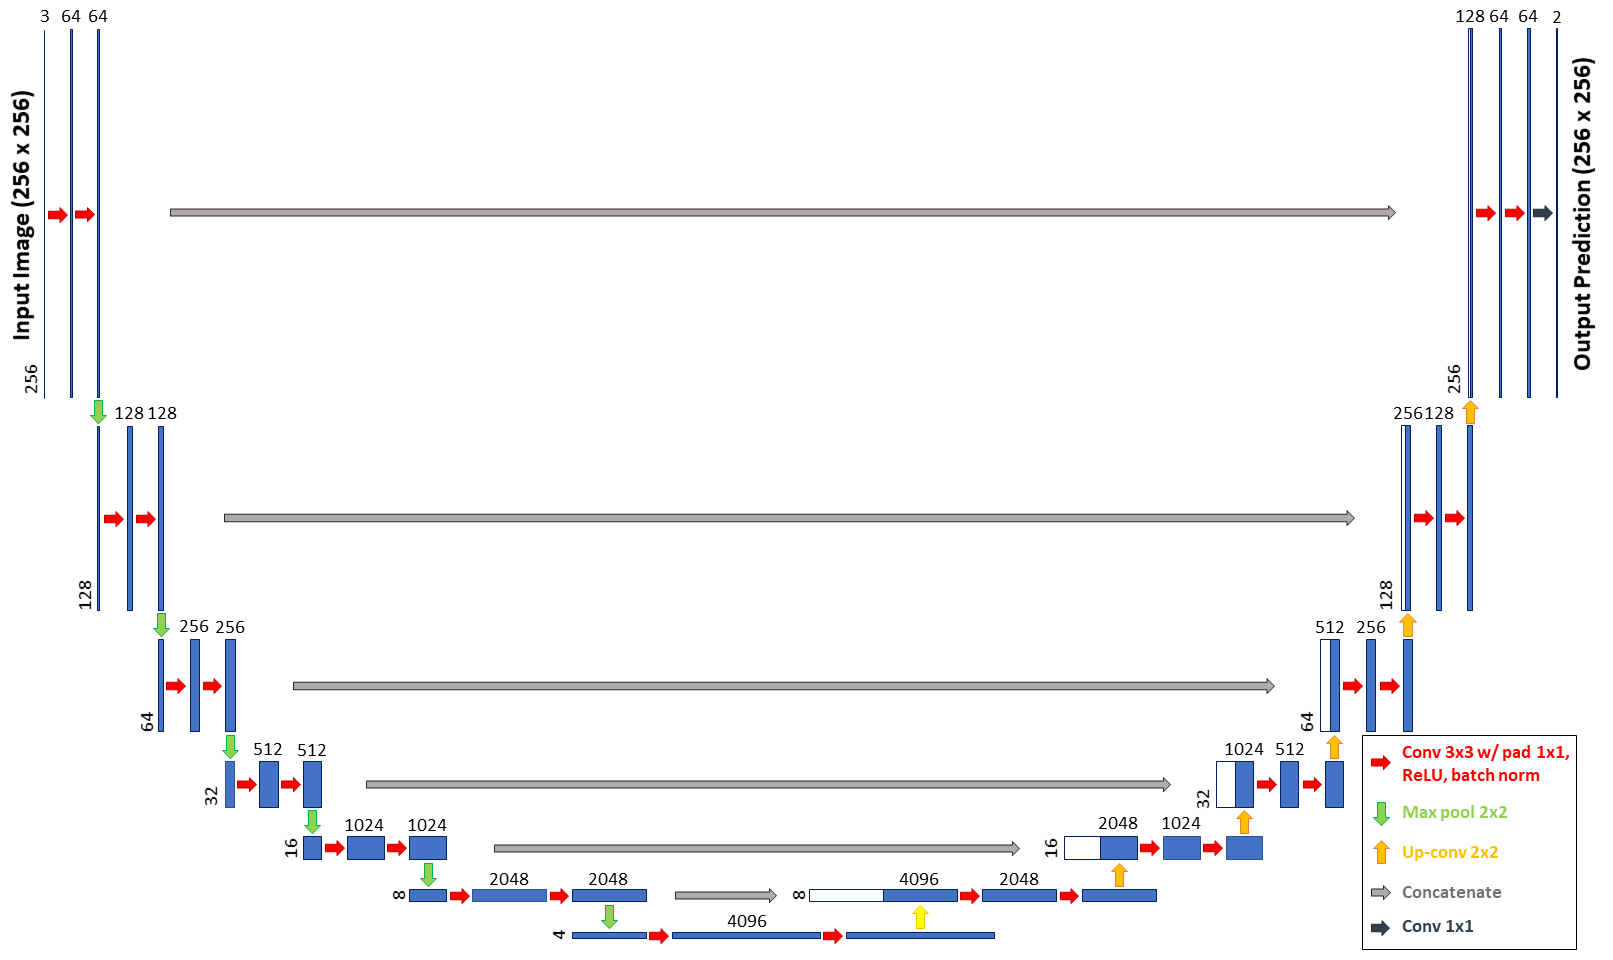
\includegraphics[width=0.7\linewidth]{Images/UNetModel.png}
  \caption{Structure of the UNet model that achieved the best results.}
  \label{fig:model}
\end{figure*}

\begin{table}[b]
    \caption{Caption goes here.}
    \label{tab:avail}
    \begin{tabular}{c|c|c}
        \toprule
        Year Collected & Season & Third col\\
        \midrule
        1994 & Spring & text\\
        1998 & Fall & text\\
        1999 & Spring & text\\
        2000 & Spring & text\\
        2001 & Spring & text\\
        2003 & Summer & text\\
        2004 & Summer & text\\
        2005 & Spring & text\\
        2006 & Summer & text\\
        2007 & Summer & text\\
        2008 & Spring and Summer & text\\
        2009 & Spring & text\\
        2010 & Summer & text\\
        2011 & Spring & text\\
        2012 & Spring and Summer & text\\
        2013 & Spring & text\\
        2014 & Summer & text\\
        2015 & Spring & text\\
        2016 & Summer & text\\
        2017 & Spring & text\\
        2018 & Spring & text\\
        2019 & Spring & text\\
        \bottomrule
    \end{tabular}
\end{table}

\section{Methodology}
\scott{Start with description of initial steps, I've pulled down the paragraph describing the Microsoft efforts and we should jump off from there.}

In June of 2018 Microsoft released a geospatial dataset of all building footprints in the United States that were extracted from the Microsoft Bing Maps Aerial and Satellite Imagery\cite{Microsoft2019}. According to the provided documentation, Microsoft then used ResNet34 and RefineNet for per-pixel building identification with their own method of polygonizing the building footprints. Although these initial results were released in mid-2018, at the time of this writing the Microsoft polygonization code and trained models have yet to be made publicly available. Our aim was to develop a system to reproduce the capabilities of the Microsoft workflow on an arbitrary set of image data that could then enable the exploration of higher resolution data sets, data sets at different epochs, and could be trained to detect different features of interest in geospatial imagery. This project hopes to replicate the Microsoft workflow to enable building detection using other, higher pixel resolution and more recent open orthophotography datasets.\footnote{Our source code (Accessed 12/11/19):\\ \url{https://github.iu.edu/ResearchApplicationsDeepLearning/BuildingFootprints}}.

\scott{The code referenced above will need to be cleaned up, quasi documented and boilerplated with a license and IU ownership and put in a public repo. The URL should be changed to that public repo when it's up}

As an initial first step we took data obtained in 2016 of Hamilton County, Indiana and prepared it to train a simple segmentation model.  \scott{pull in text from "data" section and add Jefferson's text here}
As a first attempt we undertook a segmentation using the CNN Segnet. There was a convenient implementation of Segnet in MATLAB, which allowed us to quickly train the model and see what accuracy this model would be able to achieve. Without any fine tuning, the default Segnet model returned a mean accuracy of $0.6422$ and a mean Intersection over Union (IoU) of $0.3879$. While these results are not necessarily impressive, this was a CCN with only two encoding layers and we had done no real hyperparameter tuning. This suggested that a deeper CNN with more training data would should be capable of fairly accurate building detection.

\subsection{Data}
 The data used was captured in 2016 for a portion of Hamilton County, Indiana, and contained 3-channel RGB orthophotography \cite{ISDP} in conjunction we used a corresponding grayscale image consisting of a mask for the building labels. The dataset encompassed a mostly urban setting. The grayscale image is comprised of pixel values 255 denoting a building and 0 denoting a non-building. The orthophotography has a pixel resolution of 1 ft. We cut out 256x256 GeoTIFF images from the orthophotograph and corresponding grayscale image to be used for training, validation, and testing. The option of augmentation is provided, and the number of augmented images created can be adjusted in our program. Augmentation consisted of randomly flipping the images and corresponding labels vertical and horizontally. The amount of data we used was 11,680 training images and labels, 3,960 validation images and labels, and 3,960 test images and labels.

\scott{Here we should pull apart the approach (using Matlab, then Unet, trying RefineNet, etc. from the actual tuning. Those numbers should go into the results section}
\subsection{Model}
Following the initial attempts using Segnet in MATLAB, we moved to the UNet model, implemented in PyTorch \cite{Joris2019}. This model is based on the model used in the paper, “U-Net: Convolutional Networks for Biomedical Image Segmentation.”\cite{ronneberger2015unet} Our original motivation for using UNet was that it has performed particularly well in detecting irregular edges of anomalies in medical images. The ability to precisely cut out a region based on its classification was a desirable trait for building detection. The model’s different adjustable hyperparameters are explained on van Vugt’s GitHub page \cite{Joris2019}. He also gives a brief discussion of the model’s architecture. If the padding option is not used in the model, then the workflow we have designed will automatically pad and crop the images to achieve the same original dimensions. However, the default workflow is designed to work with 256x256 pixel images.

\subsection{Hyperparameter Tuning}
 The model was trained on a single Tesla P100 GPU on Indiana University’s Carbonate computer cluster. We used Adam\cite{kingma2014adam} for the optimizer where the learning rate started at 0.001 and after every 25 epochs the program would reduce it by a factor of 10. We used weighted cross entropy\cite{Raul2018, Pytorch2019} to calculate the loss. The non-building class had a weight of 0.5 while the building class had a weight of 1, since there were significantly more non-building pixels than building pixels in the datasets. The model ran to a maximum epoch of 80 with a training batch size of 10 and testing batch size of 5. Our best scores were achieved with a model depth of 7, model Padding, no augmentation, transposed convolutions, batch normalization, and the number of filters in the first layer equaling $2^6$. Figure~\ref{fig:model} shows the structure of our model with these hyperparameters.

\subsection{Workflow}
To train and test the model, we stripped the GeoTIFF images of their metadata. The orthophotograph's RGB pixel values were set to be in the range 0 to 1. The grayscale images’ pixel values were changed to be either 1 to denote a building or 0 to denote a non-building. We fed the training dataset into the model and tested the model on the validation dataset after every epoch. Whenever the validation loss decreased, the program saved the model’s learned parameters at the current epoch. Afterwards, we loaded in the model’s parameters that achieved the lowest loss and ran it on the test dataset. We saved the predictions as gray-scale images and calculated their metrics. The metrics we calculated were recall, precision, the f1 score, and the intersection over union (IoU). Figure~\ref{fig:metrics} shows the equations for our metrics. The precision is the fraction of building pixels that were predicted correctly out of all the predicted building pixels, and recall is the fraction of building pixels that were predicted correctly out of all the building pixels in the label. The F1 score combines precision and recall to give us a better idea towards how well our model is performing, and the IoU shows how well the prediction overlaps its label. Only the labels that had buildings in them were compared to their corresponding predictions, and we used the average of our metrics over all the predictions that were compared. The IoU gave us the best idea on how well our model was doing.

\begin{figure}
  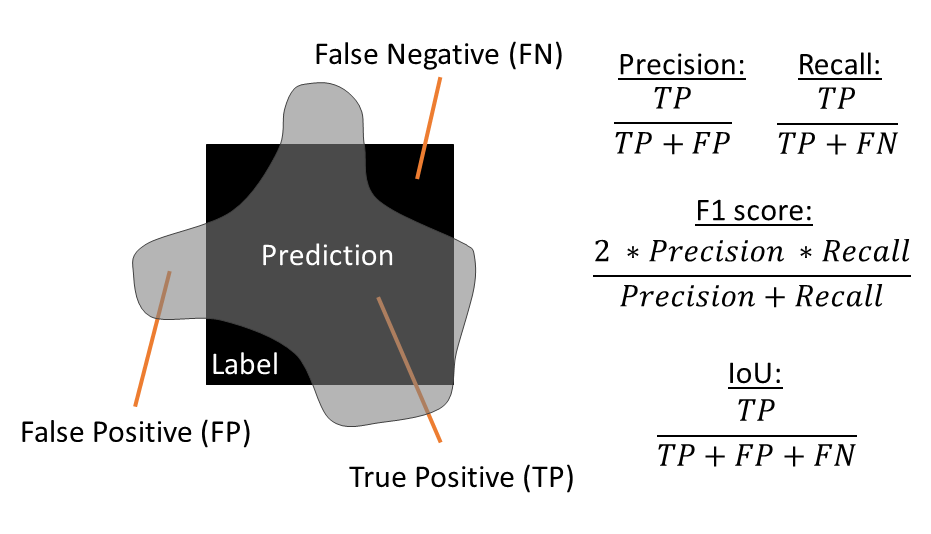
\includegraphics[width=1.0\linewidth]{Images/Metrics.png}
  \caption{Equations of the metrics used.}
  \label{fig:metrics}
\end{figure}

After obtaining the predictions from teh best model parameters, we reattached the metadata to the predictions using ExifTool \cite{Harvey2019}. We did this by copying the metadata from the orthophotograph to the corresponding grayscale predictions. We used GDAL to polygonize the new GeoTIFF images and saved them as GeoJSONs, while removing any files that did not have polygons in them as they would have been saved in an incorrect format. We fed the remaining GeoJSONs into an ogr2ogr program where their lines were smoothed using a distance tolerance of 2. Afterwards, we converted the GeoJSONs back into GeoTIFFs and stripped the metadata off them to calculate their metrics again to see if there was an improvement in scores.

\section{Results}
 Table~\ref{tab:depths} reveals the change in performance of the model with different depths. There is a small increase in the F1 score, precision, and IoU as the model increased in depth. At a depth of 7 the model achieved its best scores on epoch 30, where each epoch ran for approximately 14 minutes. Table 2 illustrates the final metrics of our model with a depth of 7 achieved before and after polygonization. There is a slight decrease in all the metrics except for precision. Figure~\ref{fig:multi} gives an example of what smoothing the predictions did.

\begin{table}
    \caption{Metrics of our test dataset when we ran the model with different depths. All other model parameters were not changed between depths.}
    \label{tab:depths}
    \begin{tabular}{l|c|c|c}
        \toprule
        Metrics & Depth 5 & Depth 6 & Depth 7\\
        \midrule
        Recall & 0.8126 & 0.7977 & 0.8170\\
        Precision & 0.7615 & 0.7768 & 0.7940\\
        F1 score & 0.7862 & 0.7871 & 0.8053\\
        IoU & 0.6682 & 0.6784 & 0.6968\\
        \bottomrule
    \end{tabular}
\end{table}

\begin{figure*}
  \begin{subfigure}[h]{0.24\textwidth}
    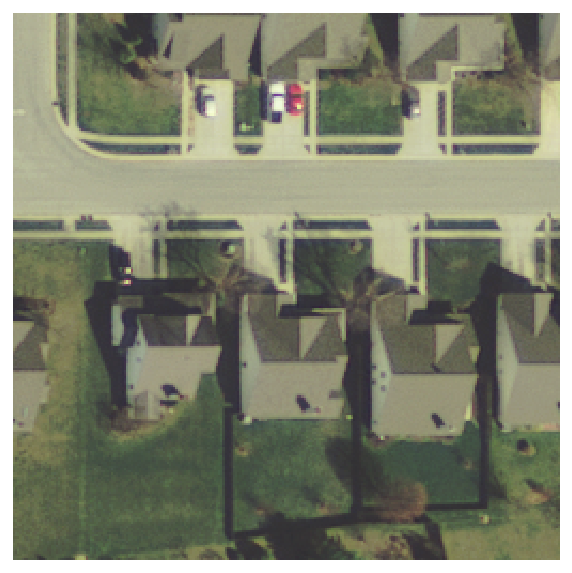
\includegraphics[width=\textwidth]{Images/0005_0028.png}
    \caption{Original orthophotograph image.}
    \label{fig:1}
  \end{subfigure}
  %
  \begin{subfigure}[h]{0.24\textwidth}
    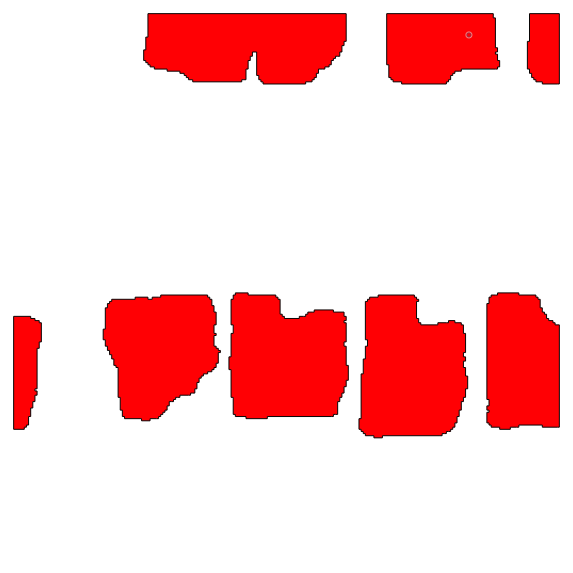
\includegraphics[width=\textwidth]{Images/0005_0028_original.png}
    \caption{Prediction in GeoJSON format.}
    \label{fig:2}
  \end{subfigure}
  %
  \begin{subfigure}[h]{0.24\textwidth}
    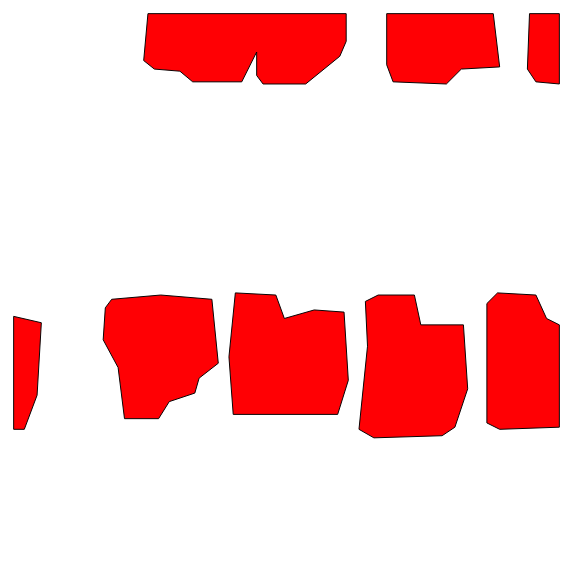
\includegraphics[width=\textwidth]{Images/0005_0028_smooth.png}
    \caption{Prediction after being smoothed.}
    \label{fig:3}
  \end{subfigure}
  %
  \begin{subfigure}[h]{0.24\textwidth}
    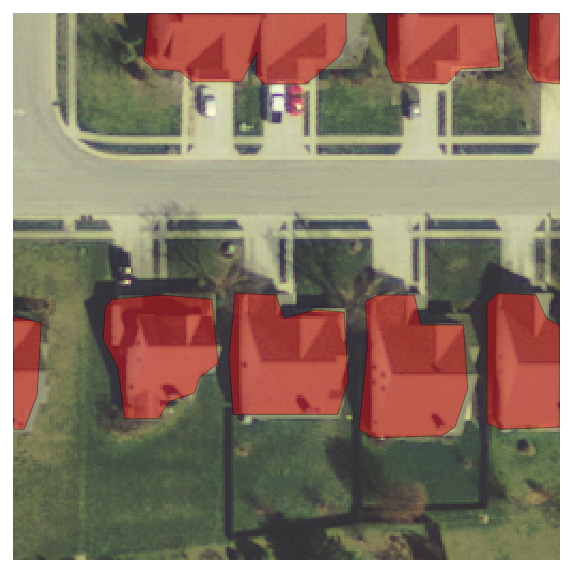
\includegraphics[width=\textwidth]{Images/0005_0028_overlap.png}
    \caption{Prediction overlapping original.}
    \label{fig:4}
  \end{subfigure}
  \caption{The before and after of smoothing the predictions.}
  \label{fig:multi}
\end{figure*}

Table~\ref{tab:obfvsmbf} also compares our results with Microsoft’s. Microsoft performed better than us in all the metrics for a few reasons. First, their training dataset consisted of 5 million training images\cite{Microsoft2019}, significantly larger than ours. It covered mostly diverse residential areas with samples of mountains, beaches, forests, etc\cite{Microsoft2019}. Also, their evaluation set consisted of 15 thousand images\cite{Microsoft2019}. They used ResNet34 and RefineNet\cite{Microsoft2019}, while we used UNet. Second, their polygonization method is much more sophisticated than ours and greatly improved their precision score, while ours only increased it slightly.

\begin{table}[]
    \caption{Our test dataset metrics from our model with a depth of 7 calculated before and after polygonization vs. Microsoft’s. Microsoft’s metrics were calculated on their evaluation set.}
    \label{tab:obfvsmbf}
    \begin{tabular}{l|cc|cc}
        \toprule
         & \multicolumn{2}{p{2.6cm}|}{Our Building Footprints}
         & \multicolumn{2}{p{2.6cm}}{Microsoft's Building Footprints}\\
        Metrics & Before & After & Before & After\\
        \midrule
        Recall & 0.8170 & 0.8091 & 0.945 & 0.935\\
        Precision & 0.7940 & 0.7966 & 0.945 & 0.996\\
        F1 score & 0.8053 & 0.8028 & N/A & N/A\\
        IoU & 0.6968 & 0.6933 & N/A & 0.85\\
        \bottomrule
    \end{tabular}
\end{table}

\section{Discussion}
We observed that our model did well on residential houses but performed worse on large buildings such as large warehouses or buildings that took up most of the 256x256 images. This likely resulted from the lack of large buildings but plenty of houses in our training dataset. Additionally, the model struggled with buildings that were oriented diagonally in an image. Sometimes the model would merge two or more of the buildings together. Furthermore, the model struggled to identify buildings if they were in the shadow of trees.


\begin{itemize}
\item Possible additions to Discussion section
\item Shadows are different for time of day and season are unique to each dataset
\item Season also affects vegetation (NAIP imagery during summer)
\item Tree foliage hide features
\item Resolution varies
\item How these variables affect the training and model
\item re-usability of model with other datasets (maybe future work section?)
\end{itemize}


\begin{itemize}
\item (JP-Move the following paragraph to future work section?)
\end{itemize}
 The test area used for this study is in a growing suburban residential area in Hamilton County north of Indianapolis, IN.  Hamilton County has been the fastest growing county in Indiana for the past four years\cite{IBRC https://news.iu.edu/stories/2019/04/iub/releases/18-indiana-sees-stronger-population-growth-census.html}.  With additional open orthophotography datasets available for the same geographic area taken during many different times ranging from 1999-2019, the model has the potential to be run on multiple dated orthophotography datasets.  The resultant output datasets can then be analyzed temporally to examine how building footprints and urban sprawl has occurred in the area of interest over the last couple of decades.



The polygonization method used can be improved upon since currently it causes a slight reduction in all but one of the metrics, but it does create results that are more visually appealing. The model would perform better with more training examples that cover a wider range of building shapes and sizes. Adding rotation to augmentation might help the model perform better on buildings oriented diagonally. Additionally, our model was not any deeper due to memory restrictions. Despite this, the model performed quite well for only having 11,680 256x256 training images. The model can be expanded into learning to detect other shapes outside of finding building footprints. Currently the program cannot classify multiple objects at once, but an edit of the code can fix that.

Originally, we used a QGIS Python script to smooth the polygonised GeoJSONs, but the dependence of QGIS prevented us from running it on the supercomputer. We switched to ogr2ogr since we received the same results as we did with QGIS, and we could run it on the supercomputer. Table~\ref{tab:time} shows the amount of time the two programs took to smooth the lines. We see that QGIS was faster in both cases despite only running on a CPU, however a benefit of using ogr2ogr was being able to automate running our polygonising, smoothing, and rasterizing Python scripts on the supercomputer. Additionally, it was much easier to set up a script to run ogr2ogr than QGIS.

\begin{table}
    \caption{Speed comparison of QGIS vs. ogr2ogr when smoothing lines for 1,921 predictions.}
    \label{tab:time}
    \begin{tabular}{l| p{3.2cm}| p{3.2cm}}
        \toprule
         & Intel Xeon E5-2680 v3 CPU (seconds) & Tesla P100 GPU (seconds)\\
        \midrule
        QGIS & 79 & N/A\\
        ogr2ogr & 124 & 89\\
        \bottomrule
    \end{tabular}
\end{table}

\section{Future Work}

\section{Conclusion}


\bibliographystyle{ACM-Reference-Format}
\bibliography{BuildDLPEARC20}

\end{document}
\endinput
